\subsection{Elektrische Kraft und elektrisches Feld}

\begin{minipage}{0.4 \linewidth}
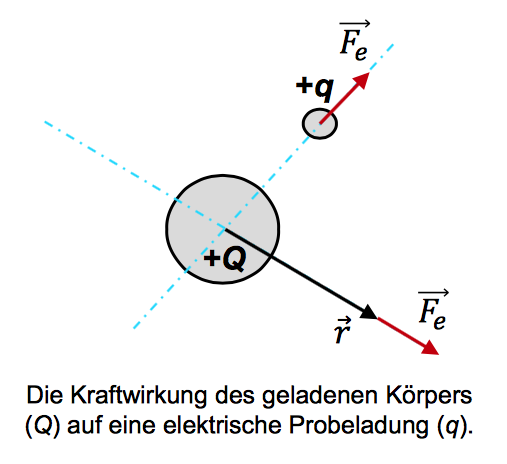
\includegraphics[width = \linewidth]{./Pics/VL1/elKraft}
\end{minipage}
\begin{minipage}{0.5 \linewidth}
Die elektrische Kraft zwischen unendlichen parallelen Leitern:

$\vec{F_{e}} = \frac{1}{2 \pi \epsilon} \cdot \frac{Qq}{r} \cdot \vec{r_{0}} (\frac{N}{m})$ \\

$\epsilon$ - dielektrische Permittivität \\
$\epsilon_{0}$ - die Permittivität des Vakuums \\
$\epsilon_{0} = 8.85 \cdot 10^{-12}$ $(\frac{As}{Vm})$ \\
$Q,q$ - Linienladungsdichten $(\frac{C}{m})$ \\
$\vec{r_{0}} = \frac{\vec{r}}{|\vec{r}|} $ - Einheitsvektor\\
\end{minipage}

\begin{minipage}{0.5 \linewidth}
Das elektrische Feld wird als die elektrische Kraft auf die Einheitsladung definiert:
\begin{equation}
\vec{E} = \frac{\vec{F_{e}}}{q} \ (\frac{V}{m})
\vec{E} = \frac{1}{2 \pi \epsilon} \cdot \frac{Q}{r} \cdot \vec{r_{0}}(\frac{V}{m})
\end{equation}
\end{minipage}
\begin{minipage}{0.4 \linewidth}
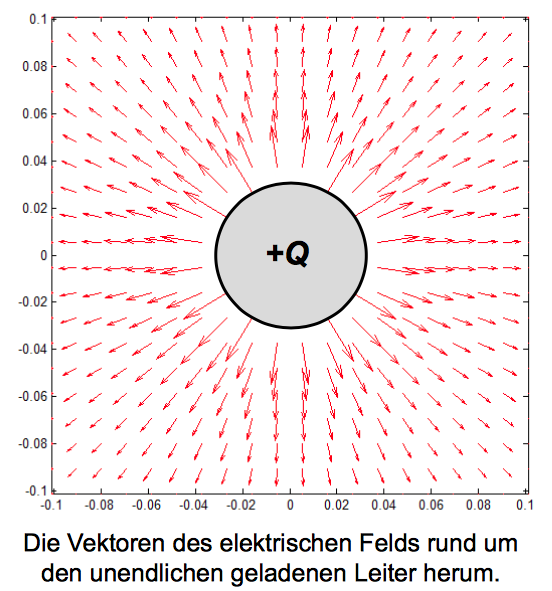
\includegraphics[width = \linewidth]{./Pics/VL1/elFeld}
\end{minipage}

\subsection{Elektrisches Potential und elektrische Spannung}

\begin{minipage}{0.5 \linewidth}
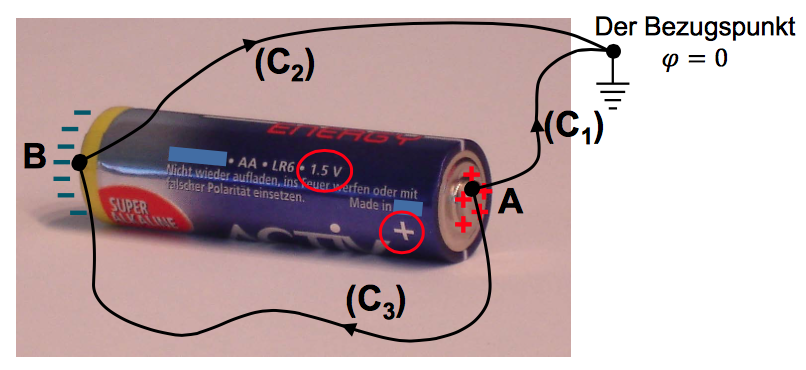
\includegraphics[width = \linewidth]{./Pics/VL1/elPot}
\end{minipage}
\begin{minipage}{0.5 \linewidth}
Die elektrische Potentiale:\\ $\varphi$ = $\int_{A}^{Bezugspunkt} \vec{E} \cdot \vec{dl}$, $\varphi_{B} = \int_{B}^{Bezugspunkt} \vec{E} \cdot \vec{dl}$
Die elektrische Spannung:
$U_{AB} = \int_{A}^{B} \vec{E} \cdot \vec{dl} = \varphi_{A} - \varphi_{B}$  (V)

Das elektrische Potential eines Ortes ist eigentlich die Arbeit, die für die Bewegung der Einheitsladung vom Bezugspunkt zum Ort nötig ist.
 \end{minipage}

\subsection{Elektrische Strom}

\begin{minipage}{0.4 \linewidth}
Elektrische Strom:

$I = \frac{dQ}{dt}$ (A)

Elektrischer Widerstand:

$R = \frac{U}{I}$  ($\Omega$)
\end{minipage}
\begin{minipage}{0.6 \linewidth}
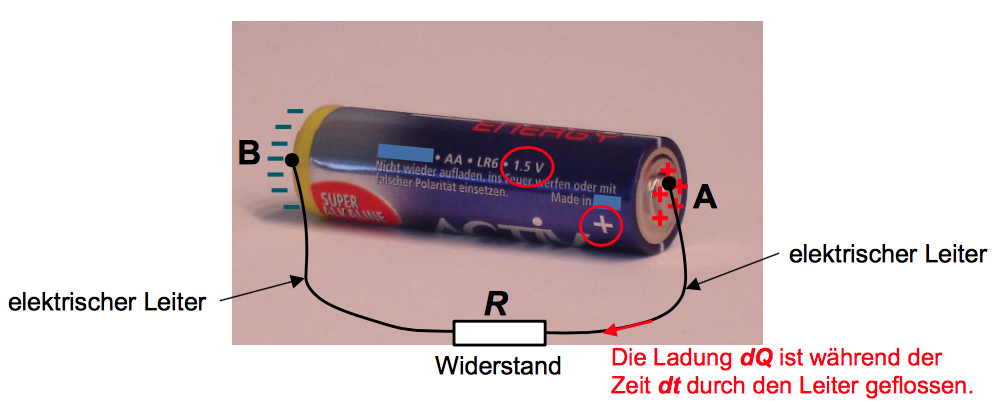
\includegraphics[width = \linewidth]{./Pics/VL1/elStrom}
 \end{minipage}
 
 \subsection{Magnetische Kraft}
 
 \begin{minipage}{0.5 \linewidth}
 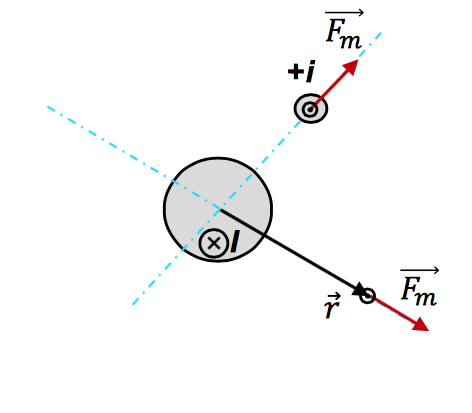
\includegraphics[width = \linewidth]{./Pics/VL1/elMag}
 \end{minipage}
 \begin{minipage}{0.5 \linewidth}
Die magnetische Kraft zwischen unendlich parallelen Leitern:
$ \vec{F_{m}} = \frac{\mu}{2 \pi} \cdot \frac{Ii}{r} \cdot \vec{r_{0}}$  ($\frac{N}{m}$) \\
$\mu$ - magnetische Permeabilität \\
$\mu_{0}$ - die Permeabilität des Vakuums \\
$\mu_{0} = 4 \pi \cdot 10^{-7}$ ($\frac{N}{A^{2}}$) \\
$I,i$ - elektrische Ströme (A) \\
$\vec{r_{0}} = \frac{\vec{r}}{|\vec{r}|} $ - Einheitsvektor \\
  \end{minipage}
  
  \begin{minipage}{0.5 \linewidth}
	Das magnetische Feld ist klein Potenzialfeld, sondern ein quellenfreies Feld: \\
	$\vec{F_{m}} = \mu \cdot i \cdot \vec{l_{0}} \times \vec{H}$  ($\frac{N}{m}$) \\
	$\vec{H} = \frac{I}{2 \pi} \cdot \frac{\vec{L_{0}} \times \vec{r_{0}}}{r}$  $(\frac{A}{m})$\\
	$\vec{r_{0}} = \frac{\vec{r}}{|\vec{r}|} $ - Einheitsvektor \\
	$\vec{L_{0}}, \vec{l_{0}}$ - Einheitsvektoren der Stromleiter \\
   \end{minipage}
   \begin{minipage}{0.5 \linewidth}
   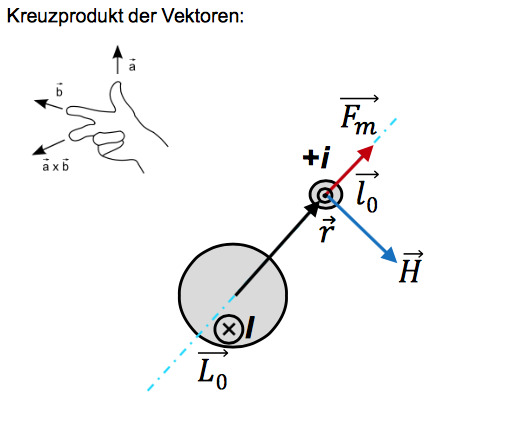
\includegraphics[width = \linewidth]{./Pics/VL1/magFeld}
    \end{minipage}
    
    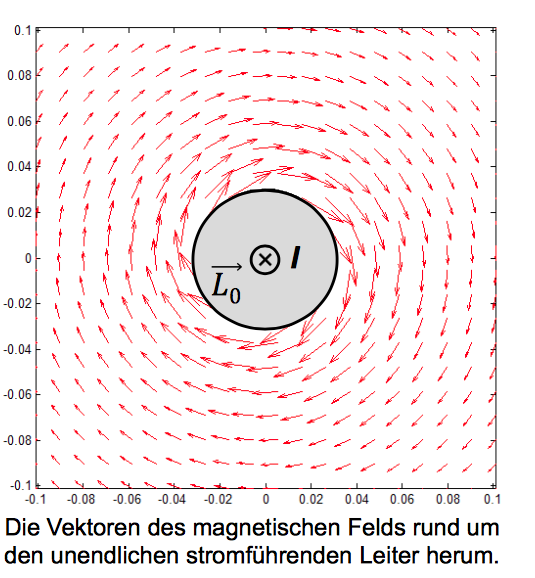
\includegraphics[width = 0.3\linewidth]{./Pics/VL1/magFeld2}
    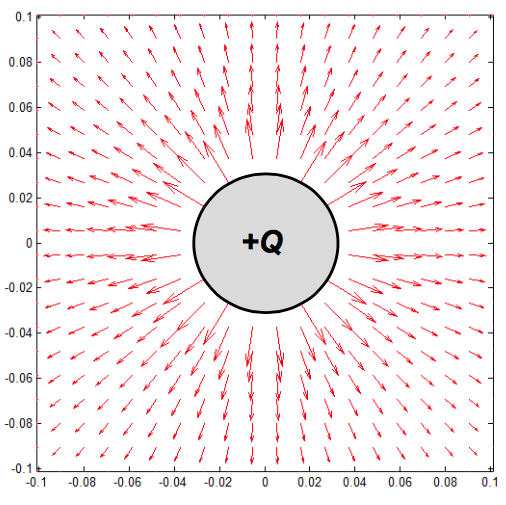
\includegraphics[width = 0.3\linewidth]{./Pics/VL1/magFeld3}
    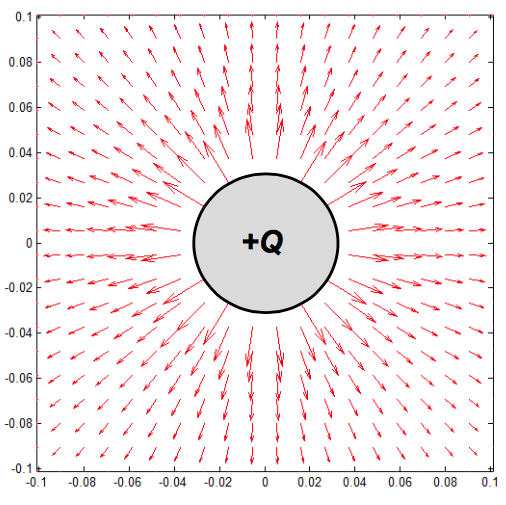
\includegraphics[width = 0.3\linewidth]{./Pics/VL1/magFeld3}
    
    $\vec{E} = \frac{1}{2 \pi \epsilon} \cdot \frac{Q}{r} \cdot \vec{r_{0}}$  ($\frac{V}{m}$) \\
    $\vec{H} = \frac{I}{2 \pi} \cdot \frac{\vec{L_{0}} \times \vec{r_{0}}}{r}$  $(\frac{A}{m})$\\
    	
\subsection{Elektrische und magnetische Kraft im Vergleich}
    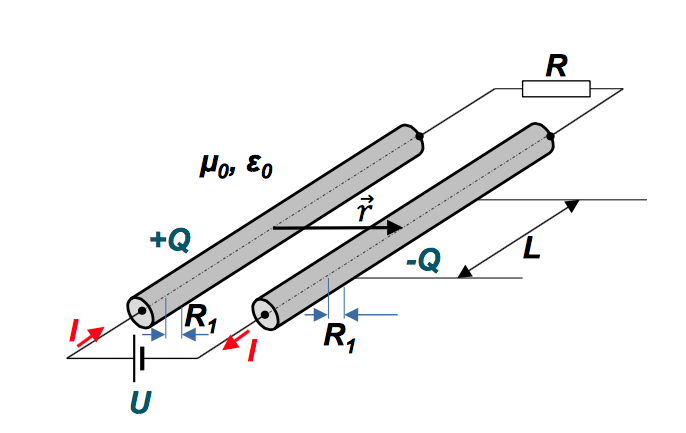
\includegraphics[width = 0.35\linewidth]{./Pics/VL1/elMagVergleich}
    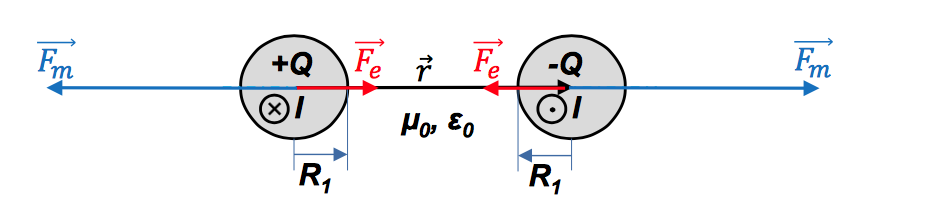
\includegraphics[width = 0.6\linewidth]{./Pics/VL1/elMagVergleich2}
    
\subsubsection{Berechnungsbeispiel}
\begin{tabular}{ll}
Die wichtige Annahme: & $r >> R_1$ \\
Die geometrischen Daten: & $R_{1}$ = 10mm, r = 100mm, L = 1000mm\\
Die elektrischen Daten:& U = 1V, I = 1A  \\
Die Kräfte pro Längeneinheit: &$F_{e} = \frac{\pi \cdot \epsilon_{0} \cdot U^{2}}{2 \cdot r \cdot (ln\frac{r-R_{1}}{R_{1}})^{2}} = 2.88 \cdot 10^{-11}$ $(\frac{N}{m})$ \\
&$F_{m} = \frac{\mu_{0} \cdot I^{2}}{2 \cdot \pi \cdot r} = 2.00 \cdot 10^{-6}$ $(\frac{N}{m})$ \\
\end{tabular}

Die wichtigsten Schlussfolgerungen:
\begin{enumerate}
\item Der Absolutbetrag der magnetischen Kraft pro Längen- und Stromeinheit ist ungefähr $7 \cdot 10^{4}$ mal grösser als der entsprechende Betrag der elektrischen Kraft pro Längen- und Spannungseinheit.
\item Um die Kraft von 1 ($\frac{N}{m}$) in dieser Anordnung zu erzeugen ist entweder der Strom von ungefähr 700A oder die Spannung von ungefähr 600'000 V notwendig. 
\item \textbf{Die Argumente 1 und 2 deuten darauf hin, dass die magnetische Kraft für die Energieumwandlung besser als die elektrische Kraft geeignet ist.} Deswegen basieren die modernen elektrischen Maschinen hauptsächlich auf der magnetischen Kraft.
\end{enumerate}
    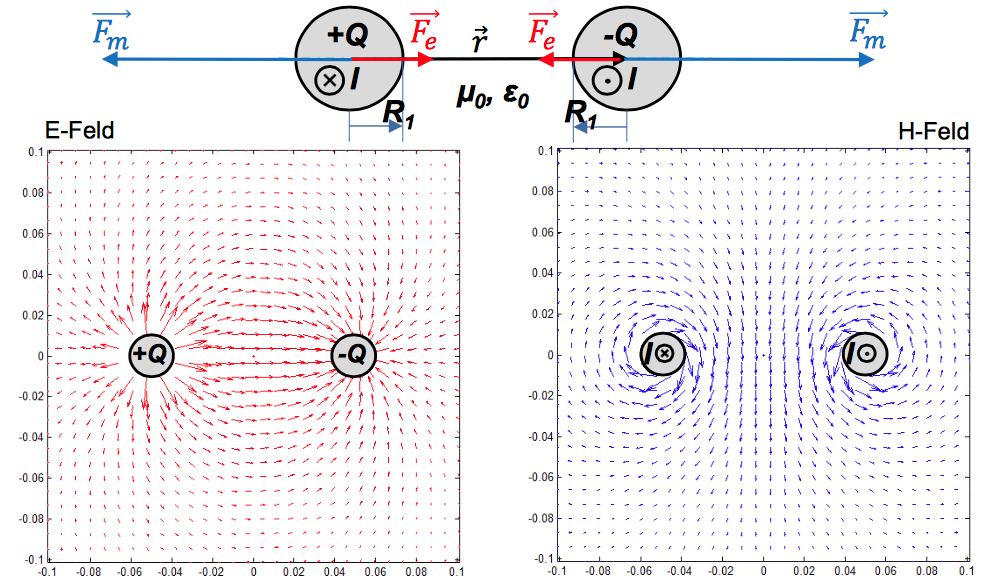
\includegraphics[width = 0.75\linewidth]{./Pics/VL1/magKraft}
    
\subsection{Begriffe und Kennwerte des Magnetfelds}
\begin{minipage}{0.2 \linewidth}
    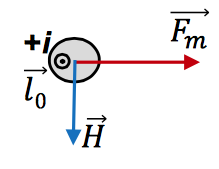
\includegraphics[width =\linewidth]{./Pics/VL1/magKraft2}
\end{minipage}
\begin{minipage}{0.8 \linewidth}
Die Kraft auf den stromführenden Leitern im Magnetfeld:\\

$\vec{F_m} = \mu \cdot i \cdot \vec{l_0} /times \vec{H}$  $(\frac{N}{m})$ = $ i \cdot \vec{l_0} \times \vec{B}$  ($\frac{N}{m}$) \\

Die magnetische Kraft ist nicht nur vom H-Feld abhängig, sondern die magnetische Eigenschaft des Materials spielen dabei auch eine wichtige Rolle. Deswegen wird \textbf{die magnetische Induktion} und \textbf{die magnetische Flussdichte} definiert:\\

$ \vec{B} = \mu \cdot \vec{H} = \mu_0 \cdot \mu_r \cdot \vec{H}$  ($T = \frac{Vs}{m^2}$) \\

$\mu_0 = 4 \pi \cdot 10^{-7}$  ($\frac{Vs}{Am} = \frac{Tm}{A}$) \\

$\mu_r = \frac{\mu}{\mu_0}$ - die relative Permeabilität des Materials \\
\end{minipage}

\begin{minipage}{0.2 \linewidth}
    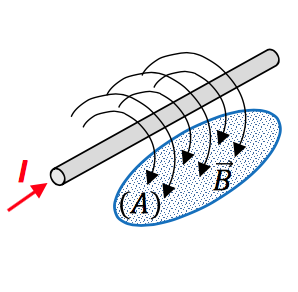
\includegraphics[width =\linewidth]{./Pics/VL1/magFluss}
\end{minipage}
\begin{minipage}{0.8 \linewidth}
\textbf{Der magnetische Fluss} ist als der Fluss des Vektors $\vec{B}$ durch eine Fläche A definiert:\\

$\Phi = \int\int_{(A)} \vec{B} \cdot \vec{dA}$ \\

Wenn der Fluss $ \Phi$ durch eine Spuhle mit $N$ Windungen fliesst, wird der gesamte Fluss der Spule denn als \textbf{der verkettete magnetische Fluss} gennant: \\

$\Psi = N \cdot \Phi$ \\

Der zeitvariierende magnetische Fluss durch eine Spule mit $N$ Windungen \textbf{induziert die folgende elektrische Spannung} in der Spule.\\

$U_{ind} = - \frac{d \Psi}{dt} = -N \frac{d \Phi}{dt}$ (V)
\end{minipage}

\begin{minipage}{0.2 \linewidth}
    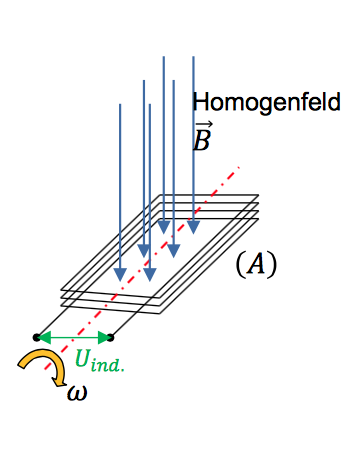
\includegraphics[width =\linewidth]{./Pics/VL1/elGen}
\end{minipage}
\begin{minipage}{0.8 \linewidth}
\textbf{Das Wirkungsprinzip eines elektromagnetischen Generators} ist hier dargestellt. Der Generator besteht im Wesentlichen aus einer Spule mit $N$ Windungen, die sich im magnetischen Homogenfeld um ihre Achse mit der konstanten Winkelgeschwindigkeit $\omega$ dreht:\\

$\Psi (t) = N \cdot \int\int_{(A)} \vec{B} \cdot \vec{dA} = N \cdot B \cdot A \cdot cos(\omega t) $ \\

\textbf{Die induzierte Spannung} der Spule kann wie folgt gerechnet werden: \\

$U_{ind.} = - \frac{d\Psi}{dt} = \omega \cdot N \cdot B \cdot A \cdot sin(\omega t)$  $(V)$
\end{minipage}

\subsection{Zusammenfassung}

\begin{itemize}
\item Die elektrische Kraft wirkt auf eine elektrische Ladung im elektrsichen Fremdfeld.
\item Die magnetische Kraft wirkt auf einen stromführenden Leiter im magnetischen Fremdfeld.
\item Die magnetische Kraft zwischen zwei parallelen stromdurchflossenen Leitern pro Strom- und Längeneinheit ist viel höher als die entsprechende elektrische Kraft zwischen den Leitern pro Spannung- und Längeneinheit.
\item Der elektrische Wechselstrom erzeugt das magnetische Wechselfeld.
\item In einer Spule, die sich im magnetischen Wechselfeld befindet, wird die elektrische Wechselspannung induziert.
\end{itemize}